\documentclass[10pt,conference]{IEEEtran}
% \IEEEoverridecommandlockouts
% The preceding line is only needed to identify funding in the first footnote. If that is unneeded, please comment it out.
\usepackage{cite}
\usepackage{amsmath,amssymb,amsfonts}
\usepackage{algorithmic}
\usepackage{graphicx}
\usepackage{textcomp}
\usepackage{xcolor}

\usepackage{listings}
\usepackage{xcolor}



\newcommand\question[1]{{\color{violet}#1}}
\newcommand\todo[1]{{\color{red}#1}}


\definecolor{codegreen}{rgb}{0,0.6,0}
\definecolor{codegray}{rgb}{0.5,0.5,0.5}
\definecolor{codepurple}{rgb}{0.58,0,0.82}
\definecolor{backcolour}{rgb}{0.97,0.97,0.97}

\lstdefinestyle{mystyle}{
    backgroundcolor=\color{backcolour},
    commentstyle=\color{codegreen},
    keywordstyle=\color{magenta},
    numberstyle=\tiny\color{codegray},
    stringstyle=\color{codepurple},
    basicstyle=\ttfamily\footnotesize,
    breakatwhitespace=false,
    breaklines=true,
    captionpos=b,
    keepspaces=true,
    numbers=left,
    numbersep=5pt,
    showspaces=false,
    showstringspaces=false,
    showtabs=false,
    tabsize=2
}

\lstset{
%   basicstyle=\ttfamily,
  mathescape
}



\usepackage{minted}
\usepackage{hyperref}


\bibliographystyle{ieeetr}

\def\BibTeX{{\rm B\kern-.05em{\sc i\kern-.025em b}\kern-.08em
    T\kern-.1667em\lower.7ex\hbox{E}\kern-.125emX}}
\begin{document}

\title{Hardware and Software Codesign for Sparse Linear Algebra Operations Acceleration 
}

\author{\IEEEauthorblockN{Aleksey Tyurin}
\IEEEauthorblockA{\textit{Saint Petersburg State University} \\
Saint Petersburg, Russia \\
alekseytyurinspb@gmail.com}
\and
\IEEEauthorblockN{Daniil Berezun}
\IEEEauthorblockA{\textit{Saint Petersburg State University} \\
\textit{JetBrains Research}\\
Saint Petersburg, Russia \\
daniil.berezun@jetbrains.com}
\and
\IEEEauthorblockN{Semyon Grigorev}
\IEEEauthorblockA{\textit{Saint Petersburg State University} \\
\textit{JetBrains Research}\\
Saint Petersburg, Russia \\
s.v.grigoriev@spbu.ru}
}


\maketitle

%% Abstract
%% Note: \begin{abstract}...\end{abstract} environment must come
%% before \maketitle command
\begin{abstract}

In the era of big data, computations are expected to be faster and less power-consuming in order to become more effective and affordable.
% Sparse linear algebra is a great framework for building algorithms in a uniform and optimization-amenable way.
% However, CPUs and GPUs currently running such algorithms are underutilized due to being too general-purposed for problems that include sparsity.
% Thus, an application-specific integrated circuit could speed sparse computations up, following the example of \textit{Google TPU's}.
% It is worth noting that such a circuit needs to be not self-contained to allow some expected optimizations to be made by a compiler or a framework itself.
% Finally, the optimizations should be easily definable in the language and as automated as possible, thus a careful simultaneous design of hardware and software is needed.
% The proposal describes the bottlenecks inherent to present sparse linear algebra framework implementations, summarizes the expected optimizations, and proposes a co-design approach to designing a highly-optimized sparse linear algebra framework.
% \textit{This is a work in progress and not yet present the final result}.

% While GPU utilization allows one to speed up computations to the orders of magnitude, memory management remains the bottleneck making it often a challenge to achieve the desired performance. Hence, different memory optimizations are leveraged to
% reduce the number of memory transactions and 
% make memory being used more effectively.
%Notably, memory optimizations are being the most significant problem: GPUs memory hierarchy implies certain limitations, thus making data memory allocation management nontrivial and memory to be utilized carefully.
%In the paper we propose an approach automating memory management utilizing partial evaluation, a program transformation technique that enables the data accesses to be precomputed, optimized, and embedded into the code, mitigating memory transactions.
% We propose an approach automating memory management utilizing partial evaluation, a program transformation technique that enables data accesses to be pre-computed, optimized, and embedded into the code, saving memory transactions.
%As an empirical evaluation of our approach we applied the technique to a straightforward CUDA C na\"ive string pattern matching algorithm implementation.
%Our experiments show that the transformed program is up to 8 times as efficient as the original one.
% An empirical evaluation of our approach shows that the transformed program could be up to 8 times as efficient as the original one in the case of CUDA C na\"ive string pattern matching algorithm implementation.   
\end{abstract}
\footnotetext{\url{https://developer.nvidia.com/cusparse} (Accessed 09.02.2021)}


\section*{Introduction}
Linear algebra is a great instrument for solving a wide variety of problems utilizing matrices and vectors for data representation and analysis with the help of highly optimized routines.
And whilst the matrices involved in a vast diversity of modern applications, e.g., recommender systems~\cite{gupta2020architectural,amazon} and graph analysis~\cite{graph1,graph2}, consist of a large number of elements, the major part of them are zeros.
Such a high sparsity incurs both computational and storage inefficiencies, requiring an unnecessarily large storage, occupied by zero elements, and a large number of operations on zeroes, where the result is obviously known beforehand.
The traditional approach to address these inefficiencies is to compress the matrix and store only the non-zero elements. 
Thus, the effect of matrices tending to be sparse in many applications makes the techniques of matrix compressed representation and sparse linear algebra to be the effective way of tackling problems in areas including but not limited to graph analysis~\cite{GAILLA}, computational biology~\cite{compBio} and machine learning~\cite{Kepner_2017}.


\begin{figure}[t]
  \centering
  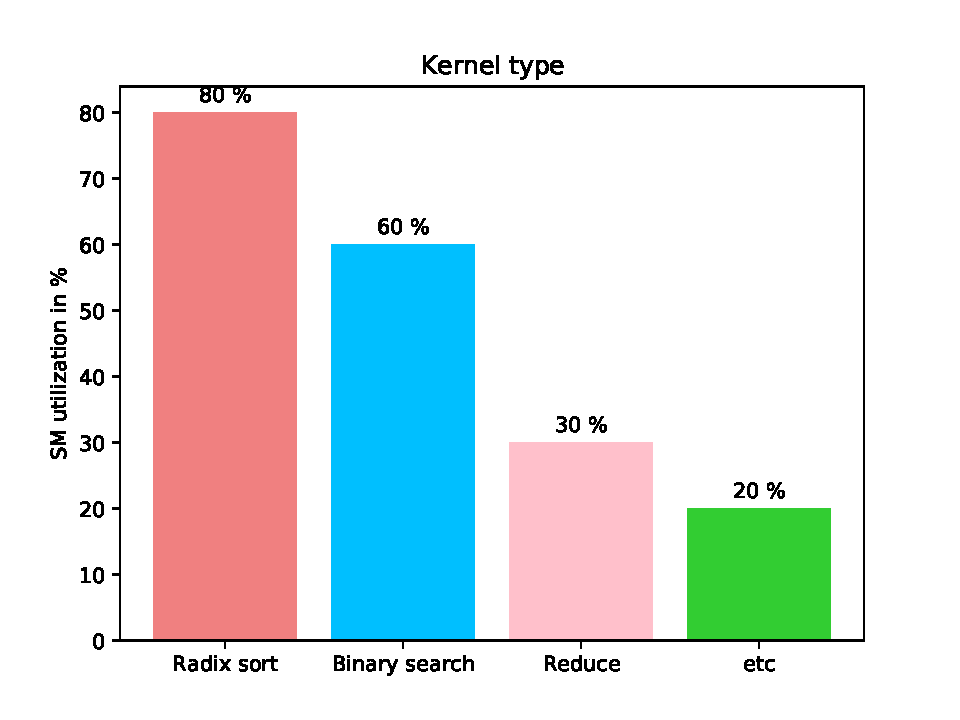
\includegraphics[width=\linewidth]{figs/SM_performance.pdf}
  \caption[Caption for LOF]{GPU's SM utilization for spMspM pipeline from cuSPARSE\footnotemark}
  \label{fig:sm_util}
\end{figure}


Sparse linear algebra defines primitives for expressing algorithms for the mentioned areas in a uniform way in terms of sparse matrix and vector operations parameterized by a semiring.
Such uniform representation allows to tune the whole bunch of expressible algorithms through optimizing the primitives solely.
One of the most used primitive is a sparse matrix-sparse matrix multiplication (spMspM) operation. 
It has finely-tuned implementations for both CPU and GPU, which, however, are proven to be underutilized due to the memory-bound nature of sparse computations induced by compressed representation~\cite{Florida,leskovec2016snap,Song_2016,zhang2020sparch}.
Further, the pipeline of spMspM is patchy, which makes some of the computational units to be idle from time to time as it could be seen in~\ref{fig:sm_util}, while the peak FLOPS is less than 1\% of maximum available. 


This makes the typical CPUs and GPUs not well-suited hardware for sparse computations and gives a rise to specialized hardware accelerators, which are primarily concerned with spMspM.
However, for a sparse framework to be useful, it should incorporate not only spMspM, but also other sparse operations parameterized by a semiring, e.g., masking, which filters the matrix elements or element-wise operations needed for, e.g., PageRank and bread-first search (BFS) algorithms~\cite{yang2020graphblast}.
And when such operations are chained explicitly or implicitly, via a loop body, certain optimizations could be applied. 
Unfortunately, some of such optimizations are only expressible at software level, i.e., in programming language, hence modern spMspM accelerators could be impractical for accelerating the whole program representing a linear algebra based algorithm like PageRank or BFS, due to the lack of a software part and to a too narrow hardware specialization.
Thus a co-design of dedicated hardware and software components, i.e., domain-specific processor (DSP) and a corresponding domain-specific language (DSL), could provide a system which is not more effective for spMspM than present hardware accelerators, but appear to be more effective in terms of speed and power consumption for holistic pieces of program, i.e., for chained operations, than current CPUs and GPUs implementations.
The ongoing work is devoted to the design of respective DSL, DSP, and an optimizing compiler, and this work in particular gives a brief overview of the filed, discusses the ideas and challenges behind the design. 



% \emph{Direction-based} optimization is in charge of either deciding to use sparse-vector or dense-vector operations for  matrix-vector multiplication. The current frontier during a graph traversal could grow while the mask of yet not-visited vertices becomes small, so it becomes more profitable to utilize masked dense operations instead of sparse-matrix sparse-vector operations.

% \emph{Load-balancing} optimization chooses the most suitable distribution among the workers (e.g. threads) depending on the sparsity of the operands. Or schedules the operands in a way to save computations, e.g. first merge two small arrays instead of a small and a large array in order to not extend a large array overhead throughout all the computation.

% \emph{Mask fusion}. Ahead-of-time masking could reduce the number of memory accesses in case of matrix-vector multiplication and prevent memory blow-up in case of matrix-matrix multiplication: the multiplication of two sparse matrices could produce an order of magnitude
% more nonzeroes in the output matrix compared with the two input matrices, hence the mask could limit the output number of nonzeroes, thus preventing out-of-memory errors. In order to achieve such a behavior, a mask should be fused (i.e. transformed in a single operation) with the corresponding operation for the operation to perform computations only for the elements in the mask.  

% \emph{Kernel fusion}. Mask fusion is a special case of kernel fusion. Kernel fusion is responsible for fusing arbitrary operations. In the case of functional programming fusion~\cite{fusion} could be thought of as eliminating allocation of intermediate values of function composition, most notably for lists, since they are the primary data structure of functional programming. In the listing~\ref{listing:3} append function \texttt{app} joins three lists, and fusion generates such code for function \texttt{f} that traverses each list only once. A simple motivating example for kernel fusion could be seen in listing~\ref{listing:2}. Masking, addition, and subtraction could be fused in one kernel code to prevent intermediate results allocation and redundant memory accesses for traversal for each or element-wise operation. The graph representation of operations could exploit operation properties, e.g., associative property, to perform the fusion. Further, the fusion for operations that could be represented as a composition of \texttt{map/reduce} operations are well-studied and could be effectively fused~\cite{KernelFusion,Futhark}.
% \begin{listing}
% \centering
% \caption{Fusion of function composition}
% \label{listing:3}
% \begin{minted}{haskell}
% app [] ls = []
% app (x:xs) ls = x : app xs ls

% -- call for this function

% app xs (app zs ys)

% -- is fused to the following function definition
% -- that is specialized for three lists

% f [] xs ys = g xs ys
% f (x:xs) ys zs = x : f xs ys zs

% g [] xs = xs
% g x:xs ys = x : g xs ys

% -- and a call
% f xs zs ys

% \end{minted}

% \end{listing}
% % \begin{minted}[escapeinside=||]{haskell}
% % map f (map g list) |$\equiv$| map (f |$\circ$| g) list 
% % \end{minted}


% \begin{listing}
% \centering
% \caption{Kernel fusion example}
% \label{listing:2}
% \begin{minted}{python}
% #Fusing together '+', '-', and masking
% #prevents two intermediate matrices allocation

% C<mask> = A + C - B
% \end{minted}
% \end{listing}

% \emph{Specialization}. Generally, it is a program transformation optimization~\cite{jones} that exploits the knowledge of some of the operation parameters, hence it could optimize those parts of the operation that depend on the known pieces of information. In the case of \emph{NVIDIA CUDA} specialization assigns a specialized computation per a warp, since warps could be executed independently. This technique is well-described, e.g.,  in~\cite{CUDADMA}. An example of such optimization could be a matrix-vector multiplication in some cycle where the vector remains unchanged. Hence, the vector could be embedded in the operation itself avoiding vector-specific overheads, e.g, allocation or data transfer back-and-forth from host to device. Matrix-vector multiplication is essentially a linear combination of columns where each column has a corresponding coefficient from the vector. Thus, each warp could multiply it's assigned column by the \texttt{warp\_id's} element of the vector, which could be embedded in the code of the warp itself. Such embedding is generally a huge \texttt{warp\_id} \texttt{switch} statement, which incurs almost no overhead in the case of CUDA.

% However, there are inevitable challenges both for the hardware running sparse algorithms and for the software, performing optimizations. 

% For the former, both CPUs and GPUs remain underutilized when executing sparse operations due to high cache-miss rates, limited communication between processors~\cite{Song_2016}. Sparse algorithms are inherently memory-bound and thus results in poor GFLOPs number compared to peak GFLOPs theoretically available on modern devices, namely less than $0.2\%$ of theoretical performance is achieved as reported in~\cite{leskovec2016snap, Florida}.

% For the latter, optimizations are hard to automate and perform in general. The runtime of graph kernels is dependent on the input data, so in a multiple iteration algorithm, it might be profitable to fuse two kernels in one iteration and two different kernels in a different iteration. Further, kernels are compelled to satisfy certain restriction to be fuseable: the absence of intermediate synchronization, same data access pattern, enough resources on the device to execute fused kernel. Once again, \texttt{map/reduce} kernels could be successfully fused, but it is unclear whether GraphBlas standard could be solely implemented in \texttt{map/reduce} terms. For specialization, it is better for the underlying hardware to be \emph{MIMD} for the workers to be completely independent, however GPU's architecture is \emph{SIMT} (or \emph{SPMT}), which prevents successful specialization in many cases.

% Eventually, some application-specific integrated circuits have been designed to address the issues mentioned above, that basically provide hardware units for sparse matrix-matrix or matrix-vector multiplication~\cite{zhang2020sparch, Song_2016, Systolic,CPU-FPGA}. A brief overview could be found in~\cite{zhang2020sparch}. The implementation from~\cite{zhang2020sparch} greatly outperforms CPUs (Intel MKL\footnote{\url{https://software.intel.com/content/www/us/en/develop/tools/oneapi/components/onemkl.html}}) and GPUs (cuSPARSE\footnote{\url{https://developer.nvidia.com/cusparse}}) solutions in terms of speed and power consumption. Despite high performance, such solutions do not yet provide a complete implementation of GraphBlas (or even a subset required for a concise BFS from the example) and seem to be too self-contained to split the operation into phases that could be optimized in the discussed sense. 

% Thus, a solution that combines the hardware and software in co-design fashion considering both hardware and software bottlenecks could be proposed. 
% The hardware should be general enough to allow software optimizations and the optimizations should be easily definable in the co-designed language. 
% A possible approach to tackle the design problem is to use a co-design framework~\footnote{\url{http://openasip.org/}} and TTA processor architecture, which is highly parallel and customizable (allowing, e.g., MIMD computations). 

% Currently, sparse algebra frameworks speed up graph data\-bases, e.g., RedisGraph~\footnote{https://oss.redislabs.com/redisgraph/}, computational biology and machine learning, and equipping cloud solutions that provide such services with the dedicated sparse hardware could both increase the performance of the queries and make the services more affordable by reducing power consumption following Google's TPUs~\footnote{\url{https://cloud.google.com/tpu}} example.   

\section{Problem statement}
Since sparse linear algebra applications are mostly concerned with graph problems, some of the optimizations are graph-specific~\cite{yang2020graphblast,graphIt}, e.g., direction optimization.
However, in memory-bound applications optimizations that minimize data transfer are essential. 
For example, \emph{kernel fusion} is a wide addressed optimization that fuses multiple operations into one, avoiding intermediate memory accesses, utilizing, e.g., registers to pass the data between the operations.
In the case of sparse linear algebra frameworks kernel fusion is not yet widely implemented, but most often related to fusing chained operations like
\begin{minted}[escapeinside=//]{haskell}
  D<M> = A eWiseAdd B eWiseMult C
\end{minted}
to avoid intermediate matrices construction and reduce memory accesses with masking~\cite{yang2020graphblast}.

The problem of intermediate data structures is common for functional programming
and there have been developed a number of 
optimization techniques that try to reduce intermediate 
data structures or computations, namely partial evaluation~\cite{jones}, deforestation~\cite{WADLER1990231}, supercompilation~\cite{supercompilation}, and distillation~\cite{distillation}.

These fusion family optimizations are implementation-dependent, meaning that the optimizer should have an access to the source code, which is impossible when the function is implemented solely in hardware, hence a software part is inevitable in the design.
Thus, present hardware accelerators are not general enough to implement and accelerate a whole sparse linear algebra-based program, e.g., do not provide arbitrary semiring support, and lack a software part hence leaving out essential optimizations.
General purpose devices such as GPUs are hard to perform some optimizations, e.g., fusion requires two GPU kernels to have the same memory access pattern and partial evaluation could induce some thread divergence due to SIMD nature of a GPU. We propose the co-design of \todo{???} to address the problems of optimizeability and expressibility.
We believe that a functional DSL, where an arbitrary semiring could be concisely and conveniently expressed, powered by a set of optimizers and compilable to some DSP with enough parallelism could be a good starting point in acceleration of sparse linear algebra based programs.
Next we discuss some possible hardware architectures and incurred challenges as well as high-level architecture of the proposed solution.

% LA but whole program optimization.
% Fusion and so on.

\todo{Static vs dynamic data.}
\todo{Specialization requires MIMD.}

\todo{Representation for data (formats)}

\todo{AOT vs JIT optimizations.} 
\todo{Some data become static in running time.} 


\section{Sparse LA arch}

\section{Graph processors}
\todo{Sparse Algrabra processors?}
Graph algorithms constitute a too large set to be implemented in one processor without a proper unification like sparse linear algebra. 
Nevertheless, there are a number of algorithm-specific accelerators~\cite{besta2019graph}, but the only sparse linear algebra instruction set processor is seems to be still unfinished~\cite{Song_2016},
while other sparse linear algebra accelerators~\cite{Song_2016,CPU-FPGA,OuterSpace,zhang2020sparch} are applicable only to certain operations like spMspM.
Notably, in~\cite{smash} an approach for hardware acceleration for compressed representation indexing is proposed, which is able to employ existing optimizations and could be integrated in existing software frameworks.  
However, we believe that to fully leverage fusion the indexing should be transparent in the software, which is not the case in~\cite{smash}.

\section{Partial Evaluation and Supercompilation}

Specialization on static data.
For GPU.

Partial cases for different models (array programming, stream fusion, kernels fusion)

Easy for functional languages, hard for imperative which are widely used for HPC.

Supercompiler provides all optimizations, but too hard to implement in general case. 
We can use small language to design LA library.

\section{Lambda processors}


\section{Dataflow processors}

TTA and other dataflow + MIMD

\section{Roadmap}

Library + language + compiler + hardware co-design.

Integration with application level.

Runtime code generation, staged compilation. 
Allows one to exploit dynamic data as static. 
For example, first round of supercompilation in compile time to fuse functions, and the second round in running time to specialize on some data. 


%% Bibliography
\bibliography{bib}


%% Appendix
% \appendix
% \section{Appendix}

% Text of appendix \ldots


\end{document}